\chapter{Processo di Sviluppo}

\section{Gestione di Progetto}
Si è utilizzato \textit{Git} per effettuare il versioning del codice durante lo sviluppo attraverso la piattaforma GitHub.
L’utilizzo che ne abbiamo fatto è descritto nella figura \ref{pic:workflow}: il branch di default è sempre il \textit{main}, al quale \textit{development} è sempre allineato. Ogni volta che era necessario implementare una nuova \textit{feature} veniva creato un brach da \textit{development}. Nel caso in cui debbano essere prodotti degli hotfix o risolti dei bug, essi vengono svolti su un branch che parte da \textit{development} e vi ritorna, prima di essere mergiato nuovamente su \textit{main}.

\begin{figure}[ht]
    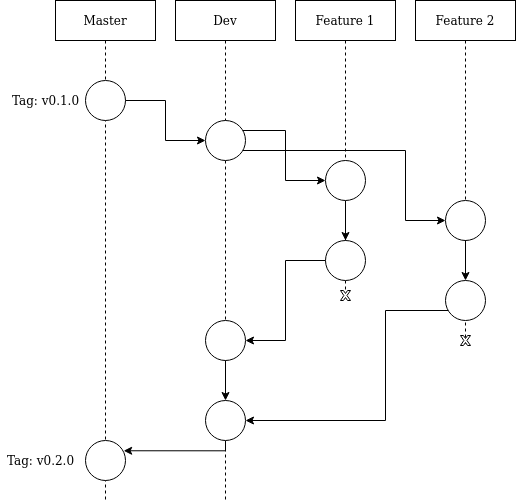
\includegraphics[width=8cm]{git-workflow.png}
    \centering
    \caption{\label{pic:workflow}Workflow del progetto.}
\end{figure}

 Successivamente, a lavoro ultimato, veniva creata una pull request per mergiare sul branch \textit{development} e infine sul \textit{main}.

\subsection{Versioning}
\subsection{Licensing}

\section{Build Automation}
La build automation è stata realizzata utilizzando il servizio delle GitHub Actions. Tutti i \textit{job} implementati venivano eseguiti sul branch \textit{development} ad ogni commit e pull-request. Inoltre i singoli \textit{job} specifici di una particolare \textit{features} venivano eseguiti anche sul branch di implementazione di quella \textit{features}. Vengono descritti tutti i \textit{job} realizzati:

\begin{itemize}
    \item \textbf{build-and-deploy-app-function}: utilizzato per deployare le \textit{azure function} in azure;
    
    \item \textbf{build-simulator}: utilizzato per eseguire la build del simulatore e creare il rispettivo \textit{artifact};
    
    \item \textbf{build-client}: utilizzato per eseguire la build del clien (lato simulatore) e creare il rispettivo \textit{artifact};
    
    \item \textbf{compile-report}: utilizzato per compilare la relazione in Latex e creare il relativo file \texttt{.pdf};
    
    \item \textbf{release}: utilizato per creare le releae del simulatore e client;
    
\end{itemize}

Inoltre sono stati implementati ulteriori due \textit{job} con lo scopo di notificarci se la build automation è terminata con successo o con un fallimento. La notifica si basa nel inviare un messaggio su un bot Telegram realizzato appositamente per il progetto (accessibile tramite questo \href{https://telegram.me/AzureHealthcareNotificator_bot}{\textit{link}}). Questi \textit{job} sono stati utilizzati nei branch \textit{development} e \textit{report}.  
\begin{itemize}
    \item \textbf{jobs-failure}: notifica tramite un messaggio sul bot Telegram che la build è fallita;  
    
    \item \textbf{jobs-success}: notifica tramite un messaggio sul bot Telegram che la build è completata con successo;  
\end{itemize}

\section{Continuos Integration}